\documentclass{standalone}

\usepackage[latin1]{inputenc}
\usepackage{amsmath}
\usepackage{amssymb}
\usepackage{amsthm}

\usepackage{tikz}
\usetikzlibrary{arrows}

%% generates a tightly fitting border around the work
%\usepackage[active,tightpage]{preview}
%\PreviewEnvironment{tikzpicture}
%\setlength\PreviewBorder{0.5mm}
%%\renewcommand\PreviewBbAdjust{-\PreviewBorder 1mm -1.15mm -0.85mm}

\usepackage{color}

%\pagestyle{empty}

\begin{document}

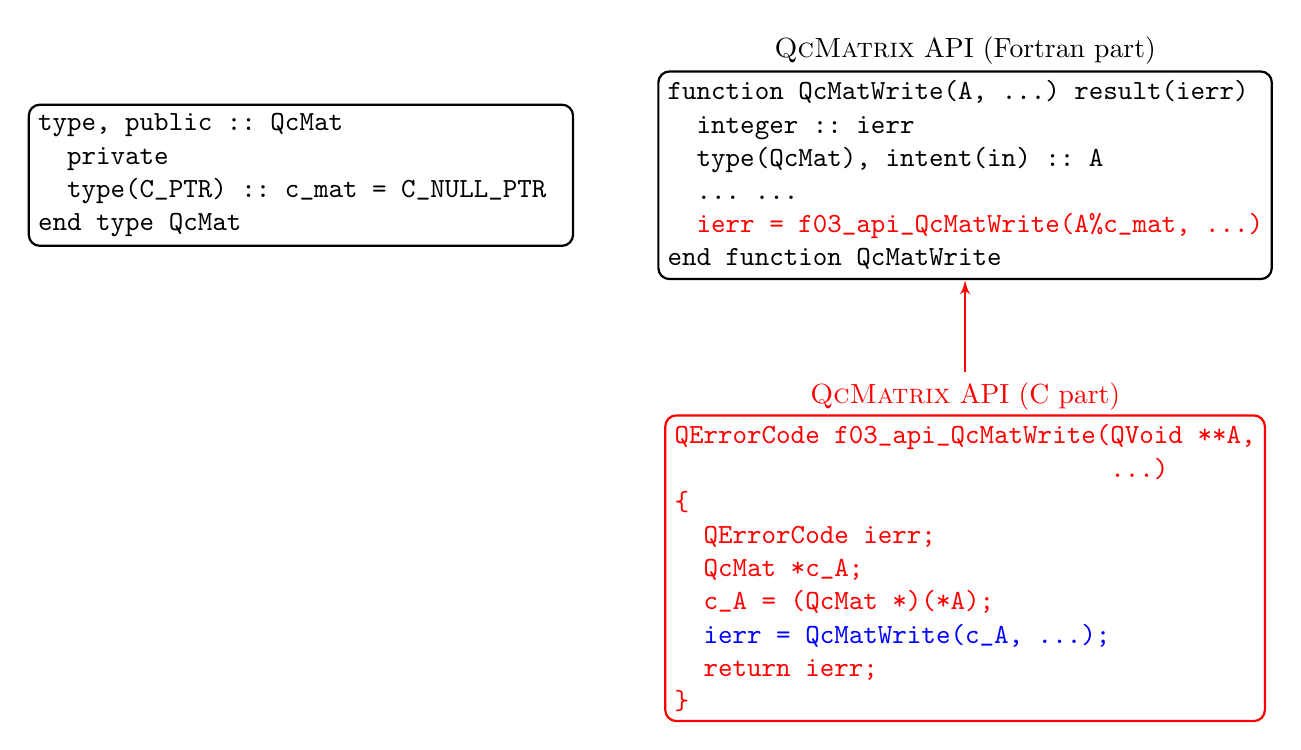
\begin{tikzpicture}[thick]
  % QcMat
  \node[color=black, rectangle, draw, text badly ragged, rounded corners, %
        minimum height=20, text width=190] (QcMatDef) %
       {\verb|type, public :: QcMat| %
        \linebreak\verb|  private| %
        \linebreak\verb|  type(C_PTR) :: c_mat = C_NULL_PTR|
        \linebreak\verb|end type QcMat|};
  % API (Fortran)
  \node[color=black, right of=QcMatDef, node distance=240, yshift=45] (NoteAPIF) %
       {\textsc{QcMatrix} API (Fortran part)};
  \node[color=black, rectangle, draw, text badly ragged, rounded corners, minimum height=20, % 
        text width=215, below of=NoteAPIF, node distance=45] (APIF) %
       {\verb|function QcMatWrite(A, ...) result(ierr)| %
        \linebreak\verb|  integer :: ierr| %
        \linebreak\verb|  type(QcMat), intent(in) :: A| %
        \linebreak\verb|  ... ...| %
        \linebreak\color{red}\verb|  ierr = f03_api_QcMatWrite(A%c_mat, ...)| %
        \linebreak\color{black}\verb|end function QcMatWrite|};
  % API (C)
  \node[color=red, below of=APIF, node distance=80] (NoteAPIC) %
       {\textsc{QcMatrix} API (C part)};
  \node[color=red, rectangle, draw, text badly ragged, rounded corners, minimum height=20, % 
        text width=210, below of=NoteAPIC, node distance=62] (APIC) %
       {\verb|QErrorCode f03_api_QcMatWrite(QVoid **A,| %
        \linebreak\verb|                              ...)| %
        \linebreak\verb|{| %
        \linebreak\verb|  QErrorCode ierr;| %
        \linebreak\verb|  QcMat *c_A;| %
        \linebreak\verb|  c_A = (QcMat *)(*A);| %
        \linebreak\color{blue}\verb|  ierr = QcMatWrite(c_A, ...);| %
        \linebreak\color{red}\verb|  return ierr;| %
        \linebreak\verb|}|};
  \draw [color=red, -latex'] (NoteAPIC)--(APIF);
\end{tikzpicture}

\end{document}
